\documentclass{beamer}
\mode<presentation> {
	\usetheme{Copenhagen}
	% remove the navigation symbols from the bottom of all slides
	\setbeamertemplate{navigation symbols}{}
}

\usepackage[T1]{fontenc}
\usepackage[utf8]{inputenc}
\usepackage{lmodern}
\usepackage{float}
\usepackage{graphicx}
\usepackage{microtype}
\usepackage{mathtools}
\usepackage{amssymb,amsmath}
\usepackage{listings}
\usepackage{biblatex}
\usepackage{hyperref}

\addbibresource{bib.bib}

\lstset{columns=fullflexible}
\newcommand{\link}[1]{{\color{blue}\href{#1}{#1}}}

\title{In-vehicle baby alert system}
\subtitle{Advanced Digital Image Processing project}
\author{F. Casciola, E. G. Ceroni, N. Landolfi} %ordine alfabetico
\institute[Unisi]{Università degli Studi di Siena}
\date{date TBD}

%Per poter compilare le slides con TexStudio, verificare che:
%1. Options - Configure TexStudio - Commands - Biber sia uguale a `biber.exe %`
%2. Options - Configure TexStudio - Build - Default Biblio Tool sia uguale a `Biber`

\begin{document}
	
	\frame{\titlepage}
	
	\section{Introduction}
	
	\begin{frame}
		\frametitle{Introduction}
		Vehicular heatstroke is largely underestimated by the general public. The majority of parents are misinformed and likely to believe that they could \textbf{never forget} their child in a vehicle.
		
		\bigskip
		
		In over 55\% of these cases, the person responsible for the child’s death unknowingly left them in the vehicle. The most dangerous mistake one can make is to think leaving a child alone in a vehicle could never happen to them.
	\end{frame}

	\begin{frame}
		\frametitle{Introduction}
		The inside of a vehicle heats up very quickly! Even with the windows cracked, the temperature inside a car can reach \textbf{51 degrees Celsius} in minutes.
		
		\bigskip
				
		A child's  body overheats three to five times faster compared to an adult, and heatstroke occurs when the body's temperature exceeds 40 degrees Celsius and the body organs begin to shut down.
	\end{frame}

	\begin{frame}
		\frametitle{Introduction: Some Data}
		\begin{figure}
			\centering
			\includegraphics[width=0.8\textwidth, height=0.8\textheight]{img/heatstroke_hist.pdf}
			\label{fig:heatstroke_hist}
		\end{figure}		
	\end{frame}

	\begin{frame}
		\frametitle{Introduction: Project Proposal}
		Based on what we have learned about Computer Vision and Image Processing, a possible solution would be to design a new system which enables \textbf{adult/child's face detection}.
		
		Even better, a hybrid solution which combines several way of measuring/sensing the child's presence would be more robust.
		
		\bigskip
		
		Our proposal is composed of three main steps:
		\begin{itemize}
			\item Collecting the data and building a dataset;
			\item Model selection and synthetic testing;
			\item Field testing of the best model.
		\end{itemize}
	\end{frame}
	
	\section{The Dataset}
	
	\begin{frame}
		\frametitle{The Dataset: Collecting The Data}
		This is the most challenging part of the project. Getting pictures of children under the age of 3 years old is not that easy.
		
		\bigskip
	
		In the beginning, we scraped images from Google Images, but we opted for a pre-existing licensed dataset \footfullcite{eidinger2014age}.
	\end{frame}

	\begin{frame}
		\frametitle{The Dataset: Sub-sampling And Dataset Adjustments}
		Since the pre-existing dataset is designed for a multi-class age classification task, we applied sub-sampling.
		
		\bigskip
		
		This yields an equal number of samples for adults and children, thus focusing the problem on a \textbf{binary classification task}.
		
		\bigskip
		
		Moreover, we decided that the images should mostly contain faces with as little background as possible. To this end, we fed our images into a face extractor\footnote{We settled for MTCNN over HAAR cascade.}.

	\end{frame}

	\begin{frame}
		\frametitle{Dataset - Definitive Version}
		Eventually, the dataset has been split in:		
		\begin{itemize}
			\item Training set: 3520 child faces and 3624 adult faces
			\item Validation set: 379 child faces and 401 adult faces
			\item Test set: 387 child faces and 238 adult faces
		\end{itemize}
	\end{frame}

	\section{Proposed Models}
	
	\begin{frame}
		\frametitle{Use-Case Overview}
		The classification task consists of 3 steps:
		\begin{enumerate}
			\item Image acquisition from a USB camera (e.g Logitech C270);
			\item Face extraction with MTCNN;
			\item Classification of the extracted faces.
		\end{enumerate}
	\end{frame}	
	
	\begin{frame}
		\frametitle{Face extractor}
		As mentioned above, we used a face extractor for two reasons:
		\begin{itemize}
			\item Training set creation: labeling faces by hand was too slow and tedious
			\item Extraction of faces from the acquired image (main use case)
		\end{itemize}
		We began with HAAR cascade, both frontal and lateral, then switched to MTCNN, which proved far superior.
	\end{frame}
	
	\begin{frame}
		\frametitle{MTCNN}
		Framework:
		\begin{itemize}
			\item Image resizing for the creation of a piramid of images
			\item The image piramid is fed to three different CNNs:
			\begin{enumerate}
				\item First, the \textbf{P-Net} produces a large number of candidate BBs\footnote{BB = Bounding box} and performs BB regression, followed by NMS\footnote{Non-maximum suppression} for merging the overlapping ones.
				\item Surviving candidates are fed to the \textbf{R-net} that performs BB regression and again NMS.
				\item At last, the survived boxes are fed to the \textbf{Q-net} that performs similarly to the R-net but it is more complicated and outputs the positions of \textbf{five facial landmarks}.
			\end{enumerate}
		\end{itemize}
	\end{frame}
	
	\begin{frame}
		\frametitle{MTCNN}
		\begin{figure}
			\centering
			\includegraphics[width=\textwidth]{img/schema_mtcnn.JPG}
    		\caption{MTCNN schematics\footfullcite{zhang2016joint}.}
    		\label{fig:schema_mtcnn}
		\end{figure}
	\end{frame}
	
	\begin{frame}
		\frametitle{Fischerface - Generalities and Training}
		Given the real-time nature of the problem we are facing, we decided to try using also a leaner method to determine wether the face in the picture belongs to a chid or an adult: Fisherface.\\ \bigskip
		During the Training phase each picture in the dataset is flattened into a single vector. After this, the PCA\footnote{Principal Component Analysis.} is performed over all the dataset, in order to find a new basis to represent our data with a reduced dimensionality\footfullcite{Belhumeur1997}.
		 
	\end{frame}
	
		\begin{frame}
		\frametitle{Fischerface - Training}
		Once the dataset is projected onto the new basis, we use it to compute the covariance matrix and the mean vector for each class. \\ \bigskip
		The covariance matrices and the mean vectors are used to find a generalised eigenvector onto which we can project the data achieving a good separation between the projections related to different classes.
		\begin{figure}
			\centering
			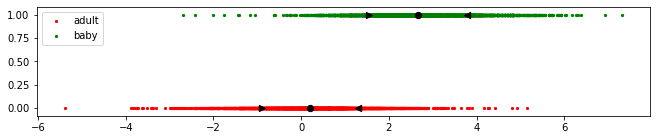
\includegraphics[width=0.8\textwidth]{img/Fisherface.png}
    		\caption{\begin{small}
    		Values of the projection onto the generalised eigenvector, the triangles indicate the first standard deviation w.r.t the mean.
    		\end{small}}
    		\label{fig:fisherface_projection}
		\end{figure}
	\end{frame}
	\begin{frame}
		\frametitle{Fischerface - Test}
		The dot product between the basis resulting from the PCA and the generalised eigenvector, we obtain a trasformation wich projects the flattened pictures directly on the latter, making this method particularly suitable for our problem. \\ \bigskip
		In the use case the pictures extracted by the MTCNN will only have to go through the following steps:
		\begin{itemize}
		\item The picture must be resized and flattened, then
		\item Projected onto the generalised eigenvector, and finally
		\item The projection has to be compared with a threshold $T$ (if it is $>T$ it will be classified as child, otherwise as adult) 
		\end{itemize}
	\end{frame}
	
	\begin{frame}
		\frametitle{Siamese Neural Network: Introduction}
		As previously mentioned, age classification is a challenging problem due to the complexity of the features that make up a face.
		
		\bigskip
		
		
		So we chose a \textbf{discriminative} approach, since we want to be able to separate \textbf{children} from \textbf{non-children}.
		
		\bigskip
		
		
		This was achieved by taking advantage of a \textbf{Siamese neural network}\footnote{Actually there is only one network that is used to process the two inputs.} that takes two inputs: a \textbf{template} image and the input image from the face extractor and checks if they belong to the same class or not. 	
	\end{frame}
	
	\begin{frame}
		\frametitle{Siamese Neural Network - The Pairs}
		This kind of neural networks require in input a pair of images:
		\begin{itemize}
			\item Template image: the class example
			\item Input image: the image that has to be classified
		\end{itemize}		
		The label $(1,0)$ symbolizes that the template image and the input image belong to the same class, $(0,1)$ otherwise.
	\end{frame}
	
	\begin{frame}
		\frametitle{Siamese Neural Network - The Pairs}
		We selected 26 child images as templates and paired them with all the other images in the original dataset\footnote{We excluded the pairs which contained the same image}, obtaining a new larger set of samples. The same procedure has been done with the adults images.
		\begin{figure}
			\centering
			\includegraphics[width=\textwidth]{img/siamese_training_set_children.JPG}
    		\caption{Siamese training - validation - test set (children network)}
    		\label{fig:siamese_general}
		\end{figure}
	\end{frame}
	
	\begin{frame}
		\frametitle{Siamese Neural Network - General Architecture}		
		\begin{figure}
			\centering
			\includegraphics[width=\textwidth]{img/siamese_schema_generale.png}
    		\caption{General outline of the network, the CNN is the same for both images}
    		\label{fig:siamese_dataset}
		\end{figure}
	\end{frame}
	
	\begin{frame}
		\frametitle{Siamese Neural Network - Discrimination module}
		The CNN part of the system actually works as an image encoder, extracting features from both the template and the input image \footnote{Could be optimized at runtime by preprocessing the templates},
		which are then fed to the \textbf{discrimination module}.
		
		The paper\footfullcite{bromley1994signature} that inspired this approach used a joining neuron that calculated the cosine distance between the encoded vectors.
		
		We decided to implement two different discriminator modules, one based on the \textbf{euclidean distance} between the CNN-encoded vectors and for the other one a \textbf{multi-layered perceptron} which was fed the concatenation of the two encoded vectors.
	\end{frame}	
	
	\begin{frame}
		\frametitle{Siamese Neural Network - Model selection strategies}
		We began our work by implementing a modified, slimmed-down version of the VGG16 architecture, based on the remarkable results that this model obtained in \textbf{ILSVRC}\footnote{ImageNet Large Scale Visual Recognition Competition} 2014.
	
		\bigskip
		
		However, we were not satisfied with the results, so we decided to build a custom network and started the cross-validation process. This however was taking too long even for a small subset of hyperparameters (although it was giving very decent results when we stopped it, see table below).
		
		\bigskip
		
		So we devised a very simple evolutionary algorithm, with accuracy on validation set as fitness function.
	\end{frame}
	
	\section{The Results}

	\begin{frame}
		\frametitle{Fisherface - Training results}
		TODO	
	\end{frame}
	
	\begin{frame}
		\frametitle{Siamese Neural Network - Training results}
		We tested the resulting networks on the appropriately\footnote{Two different sets, one for adults and one for children} held-out test set and obtained\footnote{H = Hinge loss}
		\begin{table}[]
			\centering
			\resizebox{0.8\textwidth}{!}{%
				\begin{tabular}{||c c c||}
					\hline
					Model & Accuracy & Loss  \\ [0.5ex] 
					\hline\hline
					VGG16 + MLP (Adults) & 90.43\% & 0.5991 (H) \\ 
					\hline
					VGG16 + MLP (Child) & 90.24\% & 0.5986 (H) \\ 
					\hline
					CV (Child) & 93.06\% & 0.5751 (H) \\
					\hline
					\textbf{Evo (Child)} & \textbf{94.07\%} & \textbf{0.5628} (H)  \\
					\hline
					\textbf{Evo (Adults)} & \textbf{93.46\%} & \textbf{0.5658} (H) \\ [1ex] 
					\hline
				\end{tabular}%
			}
		\end{table}
	\end{frame}
	
	\begin{frame}
		\frametitle {Siamese Neural Network - Selected architectures}
		\begin{figure}
			\centering
			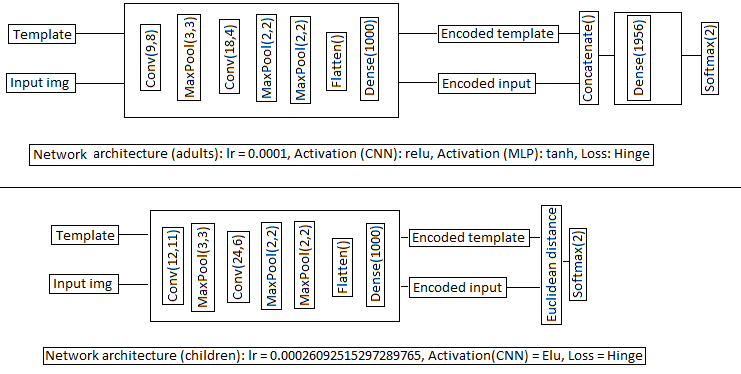
\includegraphics[width=0.9\textwidth, height=0.65\textheight]{img/schema_modelli_unico.png}
    		\caption{Selected architectures, Optimizer (both): Nadam}
    		\label{fig:selected_architectures}
		\end{figure}
	\end{frame}
	
	% TODO La section future work è meglio farla come una "sequenza" di frame
	\begin{frame}
		\frametitle{Autoencoder}
		TO BE DETERMINED
	\end{frame}
	
	\section{Conclusions}
	% TODO Parlare qui delle challange incontrati
	\begin{frame}
		\frametitle{SIFT-SURF trade-off}
		TODO trade-off tra dimensione del set di indicatori e velocità di esecuzione
	\end{frame}
	
	\begin{frame}
		\frametitle{RGB vs BGR in OpenCV}
		TODO
	\end{frame}
	
	\begin{frame}
		\frametitle{Min face dimension for MTCNN}
		TODO
	\end{frame}
	
	\begin{frame}
		\centering \Huge
		\emph{Thank You.}
	\end{frame}

\end{document}

